
Data about Facebook users and their Facebook friends are collected through our Facebook application: LinkR\footnote{LinkR homepage and application: (to be added in camera copy).}, a simple branding for ``Link Recommender''. The data collection is performed with full permission from the user and inaccordance with Ethics Protocol (to be added in camera copy). The LinkR application has the following functionalities:
\begin{enumerate}
\item Daily collection of user data.
\item Coordinating execution of recommenders for each user.
\item Provide daily recommendations of links (URLs) to users.
\item Collection of user feedback on the quality of the recommended links.
\end{enumerate}
Experiments that consisted of many different recommenders were performed between August 15th -- November 15th 2011. LinkR remains on display until its associated ethics protocol ends or no longer having research value. During this period, over 200 users installed and at any time, around 100 users are actively using LinkR. From these core LinkR users, LinkR has access to 39,850 friends, totalling 36,900 unique (and mostly private) Facebook profiles with details and interaction data. Note that data from the core users' friends are incomplete as LinkR cannot obtain their friends' data (i.e. all tracked users are one friendship link from the core users).

LinkR tracks many user (and their friends') details and interactions on Facebook. Interactions occur through wall posts provided a rich variety of content and interaction data. LinkR distinguishes four Facebook objects from wall posts: general posts\footnote{Examples: status updates, activity updates such as new friends, and interactions such as the user liked these pages.}, links, photos and videos. Four main interactions on these objects are permitted by Facebook\footnote{Some Facebook interaction features such as liking comments were introduced after LinkR user studies began and so are not tracked.}: posting object on a friend's wall, commenting, liking, and tagging. LinkR does not track deletions of these objects and interactions for performance and few deletions were observed in the initial testing of LinkR.

The tables presented distinguish the data from the core LinkR users from all the data (LinkR users and friends). Table~\ref{tab:interactions} summarises the number of records for each object and interaction combination. Table~\ref{tab:demographics} shows some demographics of the users from data collected on user profiles\footnote{Note that count of degrees are not unique as each user can attend more than one degree of the same type.}. Figures~\ref{fig:agegroups:users} and~\ref{fig:agegroups:usersfriends} show the distribution of age of users and their friends. Table~\ref{tab:history} shows some historical data in the user profiles are education and work information and the general level of detail of connections provided by Facebook. The final set of data collected by LinkR in Table~\ref{tab:interests} are important in the study of groups. This set of data provides the implicit groups of interests expressed but users (e.g. books, movies, music) and the explicit actions of users to join groups (e.g. groups with membership restrictions and pages, which essentially are groups without membership restrictions.

LinkR has collected numerous interaction and groups data for determining common preferences on Facebook. Some of these virtual interactions suggest real-world interactions as seen in photos and videos with tagging. Tagging of friends in photos and videos have some drawbacks, but we assume that tags are correct and are of real people interacting in real environments. The virtual interactions and virtual groups provide insight into Facebook communities and their diversity of topics, users and interactions with non-friends.


% 18th Jan 2012
\begin{table}
\centering
\caption{\small Number of records in Objects and Interactions Tables. Rows are type of Facebook object and columns are type of Facebook interaction.}
\label{tab:interactions}
\begin{tabular}{|>{\small}l|>{\small}r|>{\small}r|>{\small}r|>{\small}r|}
\hline
\textbf{LinkR Users} & \textbf{Posts} & \textbf{Comments} & \textbf{Likes} & \textbf{Tags} \\
\hline
\textbf{Wall} & 27,955 & 15,121 & 11,033 & 5,256 \\
\hline
\textbf{Link} & 3,974 & 5,757 & 4,279 & --- \\
\hline
\textbf{Photo} & 4,147 & 8,677 & 5,938 & 22,633 \\
\hline
\textbf{Video} & 211 & 1,687 & 710 & 2,105 \\
\hline
\hline
\textbf{LinkR Users} & \textbf{Posts} & \textbf{Comments} & \textbf{Likes} & \textbf{Tags} \\
\textbf{and Friends} & & & & \\
\hline
\textbf{Wall} & 3,384,740 & 2,152,321 & 1,555,225 & 912,687 \\
\hline
\textbf{Link} & 514,475 & 693,930 & 666,631 & --- \\
\hline
\textbf{Photo} & 1,098,679 & 2,978,635 & 1,960,138 & 8,407,822 \\
\hline
\textbf{Video} & 56,241 & 463,401 & 308,763 & 858,054 \\
\hline
\end{tabular}
\end{table}




% 18th Jan 2012
\begin{table}
\centering
\caption{\small Demographics Table}
\label{tab:demographics}
\begin{tabular}{|>{\small}p{2cm}|>{\small}r|>{\small}r|}
\hline
\textbf{Table} & \textbf{\#Records} & \textbf{\#Records} \\
& \textbf{(LinkR Users)} & \textbf{(LinkR User} \\
& & \textbf{and Friends)} \\
\hline
Users & 103 & 36,900 \\
\hline
\hline
\textbf{Column} & \textbf{\#Non-empty} & \textbf{\#Non-empty} \\
& \textbf{(LinkR Users)} & \textbf{(LinkR User} \\
& & \textbf{and Friends)} \\
\hline
Gender & 102 & 36,401 \\
\hline
Locale & 103 & 36,900 \\
\hline
Timezone & 103 & 117 \\
\hline
Birthday & 103 & 27,624 \\
\hline
Hometown\par Location & 63 & 17,584 \\
\hline
Current\par Location & 71 & 20,088 \\
\hline
\hline
\textbf{Breakdown} & \textbf{Count} & \textbf{Count} \\
& \textbf{(LinkR Users)} & \textbf{(LinkR User} \\
& & \textbf{and Friends)} \\
\hline
Male & 73 & 19,742 \\
\hline
Female & 29 & 16,659 \\
\hline
Degree:\par High School & 104 & 29,503 \\
\hline
Degree:\par College & 115 & 29,223 \\
\hline
Degree:\par Graduate School & 56 & 7733 \\
\hline
\end{tabular}
\end{table}


\begin{figure}[t!]
\centering
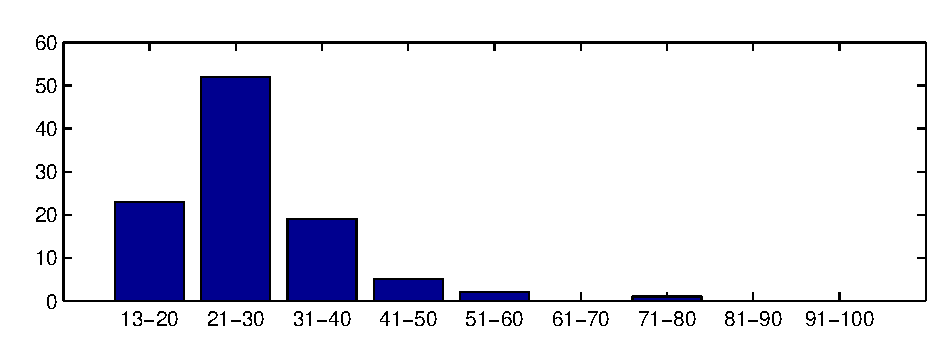
\includegraphics[scale=0.5]{data/age_groups_linkr_users.pdf}
\vspace{-15pt}
\caption{\small Number of LinkR Users by Age Groups}
\label{fig:agegroups:users}
\end{figure}

\begin{figure}[t!]
\centering
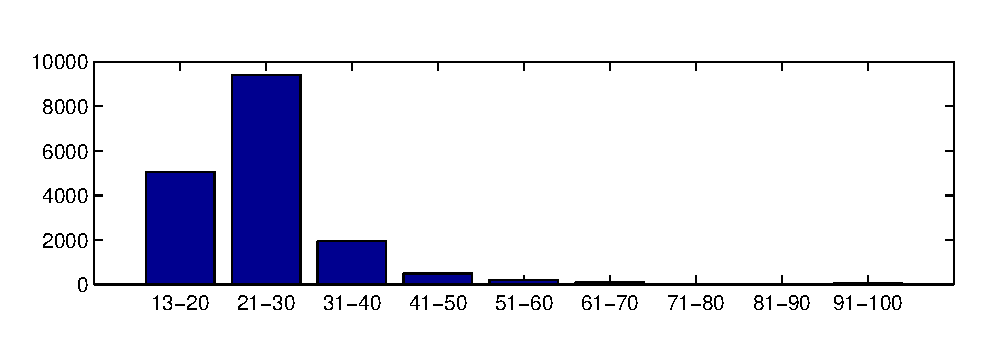
\includegraphics[scale=0.5]{data/age_groups_linkr_users_friends.pdf}
\vspace{-25pt}
\caption{\small Number of LinkR Users and Friends by Age Groups}
\label{fig:agegroups:usersfriends}
\end{figure}

\begin{comment}
\hline
Age: 11-15 & 0 & 208 \\
\hline
Age: 16-20 & 23 & 4,850 \\
\hline
Age: 21-25 & 28 & 6,257 \\
\hline
Age: 26-30 & 24 & 3,162 \\
\hline
Age: 31-35 & 10 & 1,377 \\
\hline
Age: 36-40 & 9 & 588 \\
\hline
Age: 41-45 & 4 & 293 \\
\hline
Age: 46-50 & 1 & 200 \\
\hline
Age: 51-55 & 2 & 116 \\
\hline
Age: 56-60 & 0 & 90 \\
\hline
Age: 61-65 & 0 & 60 \\
\hline
Age: 66-70 & 0 & 25 \\
\hline
Age: 71-75 & 1 & 15 \\
\hline
Age: 76-80 & 0 & 4 \\
\hline
Age: 81-85 & 0 & 11 \\
\hline
Age: 86-90 & 0 & 6 \\
\hline
Age: 91-95 & 0 & 16 \\
\hline
Age: 96-100 & 0 & 20 \\
\hline
Age: 100+ & 1 & 55 \\
\end{comment}



% 18th Jan 2012
\begin{table}
\centering
\caption{\small History Tables}
\label{tab:history}
\begin{tabular}{|>{\small}p{2cm}|>{\small}r|>{\small}r|}
\hline
\textbf{Table} & \textbf{\#Records} & \textbf{\#Records} \\
& \textbf{(LinkR Users)} & \textbf{(LinkR User} \\
& & \textbf{and Friends)} \\
\hline
Education & 275 & 66,462 \\
\hline
School & 275 & 27,635 \\
\hline
School Classes & 89 & 5,825 \\
\hline
School Class & 115 & 8,313 \\
With Friends & & \\
\hline
School Degree & 275 & 1,730 \\
\hline
School Degree & 96 & 14,429 \\
Concentration & & \\
\hline
School & 80 & 12,575 \\
With Friends & & \\
\hline
Work & 134 & 28,610 \\
\hline
Work Employer & 134 & 19,053 \\
\hline
Work Position & 134 & 7,947 \\
\hline
Work Projects & 9 & 1,336 \\
\hline
Work Projects & 0 & 4,466 \\
With Friends & & \\
\hline
Work & 21 & 5,204 \\
With Friends & & \\
\hline
\end{tabular}
\end{table}






% 18th Jan 2012
\begin{table}
\centering
\caption{\small Groups of Interests Tables}
\label{tab:interests}
\begin{tabular}{|>{\small}p{2cm}|>{\small}r|>{\small}r|}
\hline
\textbf{Table} & \textbf{\#Records} & \textbf{\#Records} \\
& \textbf{(LinkR Users)} & \textbf{(LinkR User} \\
& & \textbf{and Friends)} \\
\hline
Activities & 394 & 92,148 \\
\hline
Books & 266 & 52,690 \\
\hline
Favorite Athletes & 58 & 23,009 \\
\hline
Favorite Teams & 35 & 14,772 \\
\hline
Groups & 3,792 & 778,751 \\
\hline
Inspirational People & 39 & 7,815 \\
\hline
Interests & 153 & 36,085 \\
\hline
Movies & 616 & 149,197 \\
\hline
Music & 1,245 & 318,296 \\
\hline
Pages & 11,973 & 3,004,360 \\
\hline
Sports & 48 & 8,663 \\
\hline
Television & 819 & 144,308 \\
\hline
\end{tabular}
\end{table}





\begin{comment}
% 18th Jan 2012
\begin{table}
\centering
\caption{\small All other records.}
\label{tab:all}
\begin{tabular}{|>{\small}p{2cm}|>{\small}r|>{\small}r|}
\hline
\textbf{Table} & \textbf{\#Records} & \textbf{\#Records} \\
& \textbf{(LinkR Users)} & \textbf{(LinkR User} \\
& & \textbf{and Friends)} \\
\hline
Activities & 394 & 92,148 \\
\hline
Books & 266 & 52,690 \\
\hline
Education & 275 & 66,462 \\
\hline
Favorite Athletes & 58 & 23,009 \\
\hline
Favorite Teams & 35 & 14,772 \\
\hline
Friends & 35,869 & 39,873 \\
\hline
Groups & 3,792 & 778,751 \\
\hline
Inspirational People & 39 & 7,815 \\
\hline
Interests & 153 & 36,085 \\
\hline
Location & 206 & 6,636 \\
\hline
Movies & 616 & 149,197 \\
\hline
Music & 1,245 & 318,296 \\
\hline
Pages & 11,973 & 3,004,360 \\
\hline
School & 275 & 27,635 \\
\hline
School Classes & 89 & 5,825 \\
\hline
School Class With Friends & 115 & 8,313 \\
\hline
School Degree & 275 & 1,730 \\
\hline
School Degree Concentration & 96 & 14,429 \\
\hline
School With Friends & 80 & 12,575 \\
\hline
Sports & 48 & 8,663 \\
\hline
Sports With Friends & 26 & 3,577 \\
\hline
Television & 819 & 144,308 \\
\hline
Users & 103 & 36,900 \\
\hline
Work & 134 & 28,610 \\
\hline
Work Employer & 134 & 19,053 \\
\hline
Work Position & 134 & 7,947 \\
\hline
Work Projects & 9 & 1,336 \\
\hline
Work Projects With Friends & 0 & 4,466 \\
\hline
Work With Friends & 21 & 5,204 \\
\hline
\end{tabular}
\end{table}
\end{comment}

